%%%%%%%%%%
\subsection{Plasma screening and heavy-nuclear catalysis}\label{ssec:PlasmaScreening}
%%%%%%%%%%
The gold nanorods embedded in the NAPLIFE targets (\rsec{sssec:Anten}) and the ionized gold ``pusher'' shell (see the opto-electro-mechanical scheme \rsec{sssec:optoelecmechFusion}) share a heavy, highly-charged nucleus sitting inside a dense, laser-generated electron cloud. Independently of any accelerating field this cloud exerts, the cloud itself polarizes around the heavy ion and locally lowers the Coulomb wall seen by nearby light nuclei. This plasma screening occurs with electron densities near a $Z=79$ gold ion far from the textbook weak-field regime. It is therefore important to model this screening rigorously as it modifies fusion rates within the plasma. Refs.~\cite{Grayson:2024uwg,Grayson:2025kva} carry out this analysis first for the cosmological electron-positron plasma of Big Bang nucleosynthesis (BBN) and then for a gold ion embedded in a hot laser-produced plasma.

%%%%%%%%%%
\subsubsection{Potential-dependent screening mass}\label{sssec:ScreeningMass}
%%%%%%%%%%

Ordinary Debye-H\"uckel screening assumes the electromagnetic potential energy is everywhere small compared to the plasma temperature $T$, $Ze\phi(r)/T\ll1$, so that the induced charge density is linear in $\phi$~\cite{Barker:2002mfp}. This weak-field condition fails close to any nucleus as reacting particles tunnel at the Gamow energy, which probes distances on the of order femtometers, where $Ze\phi/T$ can vastly exceed unity. The recourse then is to then solve the Poisson equation self-consistently, keeping the full nonlinear dependence of the induced charge on the potential. Additionally, it is required to use relativistic Fermi--Dirac statistics for the electrons rather than the Boltzmann approximation, an inadequate approximation nearly universal in the older literature; see Ref.~\cite{Birrell:2024bdb} for an improved treatment.

Writing the unitless potential $\Phi\equiv e\phi/T$ and introducing a potential-dependent screening mass $m_s(\Phi)$, the rescaled Poisson equation takes the compact form
\begin{equation}\label{eq:PBscreen}
-\nabla^2\Phi(r) + \frac{m_s^2(\Phi)}{(\hbar c)^2}\,\Phi(r) = P_\mathrm{ext}(r)\,,
\end{equation}
which reduces to Debye-H\"uckel theory when $\Phi\ll1$ and to the Thomas--Fermi model as $T\to0$. In the ultrarelativistic, strong-field limit relevant near the nuclear surface the screening mass itself becomes~\cite{Elze:1980er,Kodama:2002xjg}
\begin{equation}\label{eq:screenmass}
m^2_{s,\mathrm{FD}}(\Phi) \approx \frac{4\alpha T^2}{3\pi}\left[\pi^2 + \Phi^2(r)\right]\,,
\qquad
m/\Phi T\ll 1\,,
\end{equation}
a weak-field (Debye) term plus a nonlinear correction that grows with the local potential rather than saturating exponentially as the older Boltzmann treatment predicts. Over the range probed by tunneling, see \rf{fig:ScreenMassFD}, Boltzmann statistics overestimates the screening mass, and hence the reaction-rate enhancement, by orders of magnitude relative to the correct Fermi--Dirac result.

\begin{figure}[ht]
\centering
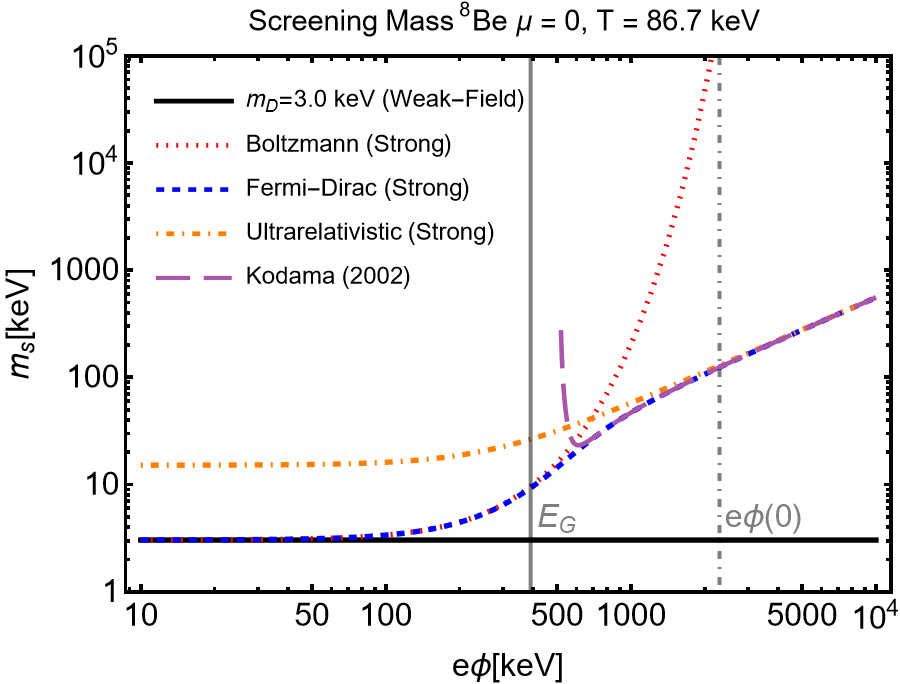
\includegraphics[width=0.72\linewidth]{ScreeningMassFD.png}
\caption{Effective screening mass $m_s$ around a finite-sized $^4$He (\,$^8$Be\,) nucleus at BBN temperature $T=86.7$~keV, as a function of the local potential $e\phi$. The self-consistent Fermi--Dirac result (blue dashed) tracks the weak-field Debye value $m_D$ (black) at small $\Phi$ but rises only as a power law at large $\Phi$; the traditionally used Boltzmann approximation (red dashed) instead diverges exponentially, over-predicting screening in the tunneling-relevant window bounded by the Gamow energy $E_G$ and the on-surface potential $e\phi(0)$. Reprinted from Ref.~\cite{Grayson:2024uwg} under \href{https://creativecommons.org/licenses/by/4.0/}{CC~BY~4.0}.}
\label{fig:ScreenMassFD}
\end{figure}

%%%%%%%%%%
\subsubsection{Fusion rate enhancement}\label{sssec:FusionEnhancement}
%%%%%%%%%%

Reaction-rate enhancement follows the Salpeter form~\cite{Salpeter:1954nc}, in which the fractional change in reaction rate is set by the induced potential evaluated at the origin
\begin{equation}\label{eq:salpeter}
\mathcal{F}_\mathrm{sc} \equiv \frac{R_\mathrm{sc}}{R_\mathrm{vac}} \sim \exp\!\left(\frac{e\phi_\mathrm{ind}(0)}{T}\right)\,.
\end{equation}
Ref.~\cite{Grayson:2025kva} applies this same self-consistent machinery to a fully ionized gold nucleus ($Z=79$) embedded in the $\sim$keV electron plasma produced when a relativistic laser pulse strips electrons from a gold nanorod or nanoparticle (a situation realized in NAPLIFE targets). Although \req{eq:PBscreen} is nonlinear, the strong-screening and weak-field (Debye) contributions to the induced potential near the origin turn out to be additive, so the weak-field part can be subtracted at each temperature to isolate a strong-screening contribution $e\phi_\mathrm{ind}(0)\simeq14.2$~keV that is independent of plasma temperature. This is close to the zero-temperature potential shift of the bound-electron cloud of a gold atom, 
\begin{equation}
    e\phi_\mathrm{HF}(0)=\alpha^2Z^{4/3}a_\mathrm{TF}m_e\simeq14.7\,\mathrm{keV}
\end{equation}
obtained from the Hartree--Fock screened-Coulomb potential shifts tabulated in Ref.~\cite{garrett1967potential} ($a_\mathrm{TF}\approx1.598$ at $Z=79$). For two light reactants of charge $Z_1,Z_2$ tunneling near a heavy catalyst of charge $Z_3$, the full multi-body enhancement factor becomes
\begin{equation}\label{eq:goldF}
\mathcal{F}_\mathrm{sc} = \exp\!\left[\frac{1}{T}\left(Z_1Z_2\,\alpha\, m_{s,\mathrm{FD}}(r_G) + Z_3\frac{Z_1+Z_2}{2}\,\alpha\, m_{s,\mathrm{FD}}(r_G) + \frac{Z_1+Z_2}{2}\,\phi_\mathrm{ind}(r_G)\right)\right]\,,
\end{equation}
evaluated at the Gamow turning point $r_G$. \rf{fig:GoldEnhance} shows the resulting enhancement for several aneutronic and near-aneutronic reactions as a function of plasma temperature. Because catalysis grows with the charge of the reacting pair, $p+{}^{11}\mathrm{B}$ benefits the most, while $d$-based reactions are enhanced more modestly.

\begin{figure}[ht]
\centering
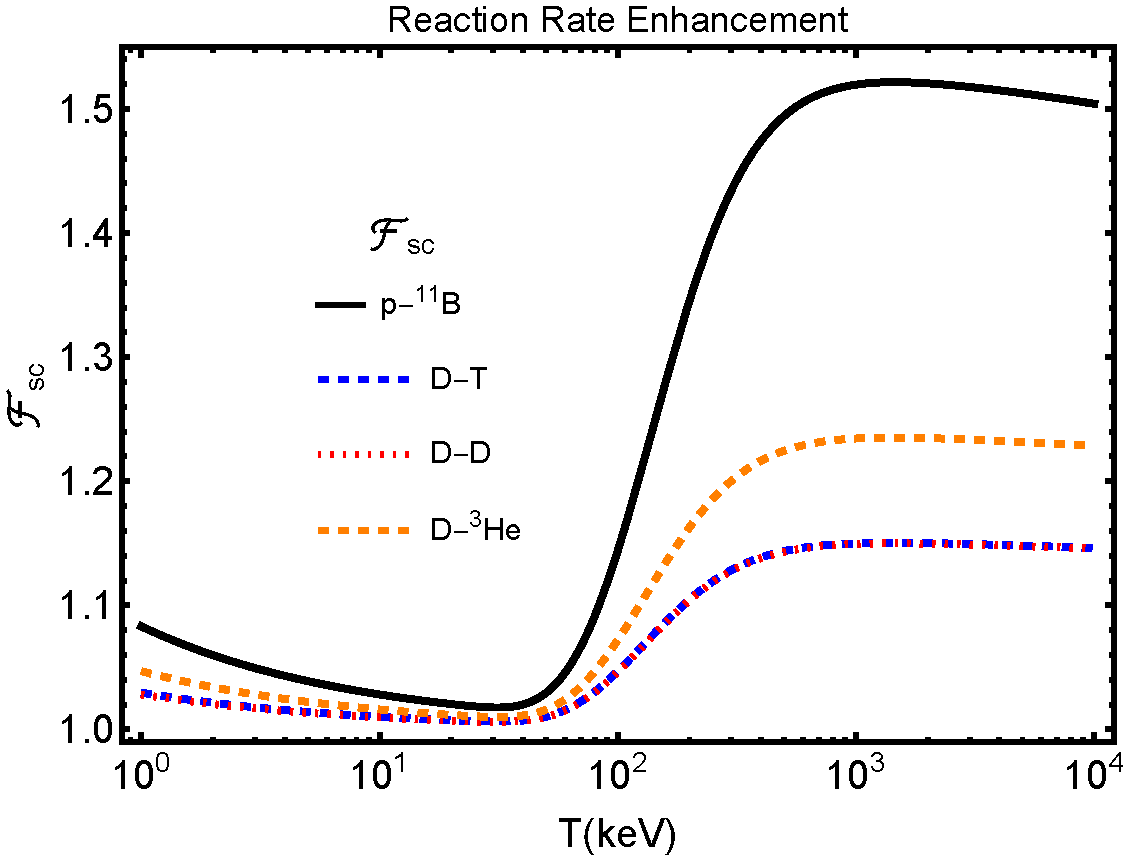
\includegraphics[width=0.72\linewidth]{ScreenEnhanceGold.pdf}
\caption{Reaction-rate enhancement factor $\mathcal{F}_\mathrm{sc}$ [\req{eq:goldF}] near a fully ionized gold catalyst, as a function of plasma temperature, for $p$-${}^{11}$B (black solid), $d$-$t$ (blue dashed), $d$-$d$ (red dotted), and $d$-${}^3$He (orange dashed). All curves rise slowly at low $T$, where the temperature-independent strong-screening term of \req{eq:screenmass} dominates, then climb sharply above $\sim100$~keV as thermal electrons increasingly penetrate the gold polarization cloud, before flattening once $T$ approaches $m_ec^2$. Reprinted from Ref.~\cite{Grayson:2025kva} under \href{https://creativecommons.org/licenses/by/4.0/}{CC~BY~4.0}.}
\label{fig:GoldEnhance}
\end{figure}

A factor of order unity is modest next to the field-acceleration mechanisms of \rsec{ssec:Plasmonics}, but it is a genuinely distinct, additive effect which requires no coherent plasmon field, but only the local electron density that any sufficiently heavy, ionized nucleus drags in a hot plasma. This may provide an explanation for the long-standing ``anomalous screening'' seen in low-energy astrophysical $S$-factor measurements~\cite{Grayson:2025kva}.
